% Options for packages loaded elsewhere
\PassOptionsToPackage{unicode}{hyperref}
\PassOptionsToPackage{hyphens}{url}
\documentclass[
]{article}
\usepackage{xcolor}
\usepackage[numbers,sort&compress]{natbib}
\usepackage{amsmath,amssymb}
\setcounter{secnumdepth}{-\maxdimen} % remove section numbering
\usepackage{iftex}
\ifPDFTeX
  \usepackage[T1]{fontenc}
  \usepackage[utf8]{inputenc}
  \usepackage{textcomp} % provide euro and other symbols
\else % if luatex or xetex
  \usepackage{unicode-math} % this also loads fontspec
  \defaultfontfeatures{Scale=MatchLowercase}
  \defaultfontfeatures[\rmfamily]{Ligatures=TeX,Scale=1}
\fi
\usepackage{lmodern}
\ifPDFTeX\else
  % xetex/luatex font selection
\fi
% Use upquote if available, for straight quotes in verbatim environments
\IfFileExists{upquote.sty}{\usepackage{upquote}}{}
\IfFileExists{microtype.sty}{% use microtype if available
  \usepackage[]{microtype}
  \UseMicrotypeSet[protrusion]{basicmath} % disable protrusion for tt fonts
}{}
\makeatletter
\@ifundefined{KOMAClassName}{% if non-KOMA class
  \IfFileExists{parskip.sty}{%
    \usepackage{parskip}
  }{% else
    \setlength{\parindent}{0pt}
    \setlength{\parskip}{6pt plus 2pt minus 1pt}}
}{% if KOMA class
  \KOMAoptions{parskip=half}}
\makeatother
\usepackage{longtable,booktabs,array}
\usepackage{calc} % for calculating minipage widths
% Correct order of tables after \paragraph or \subparagraph
\usepackage{etoolbox}
\makeatletter
\patchcmd\longtable{\par}{\if@noskipsec\mbox{}\fi\par}{}{}
\makeatother
% Allow footnotes in longtable head/foot
\IfFileExists{footnotehyper.sty}{\usepackage{footnotehyper}}{\usepackage{footnote}}
\makesavenoteenv{longtable}
\usepackage{graphicx}
\usepackage{pdflscape}
\makeatletter
\newsavebox\pandoc@box
\newcommand*\pandocbounded[1]{% scales image to fit in text height/width
  \sbox\pandoc@box{#1}%
  \Gscale@div\@tempa{\textheight}{\dimexpr\ht\pandoc@box+\dp\pandoc@box\relax}%
  \Gscale@div\@tempb{\linewidth}{\wd\pandoc@box}%
  \ifdim\@tempb\p@<\@tempa\p@\let\@tempa\@tempb\fi% select the smaller of both
  \ifdim\@tempa\p@<\p@\scalebox{\@tempa}{\usebox\pandoc@box}%
  \else\usebox{\pandoc@box}%
  \fi%
}
% Set default figure placement to htbp
\def\fps@figure{htbp}
\makeatother
\setlength{\emergencystretch}{3em} % prevent overfull lines
\providecommand{\tightlist}{%
  \setlength{\itemsep}{0pt}\setlength{\parskip}{0pt}}
\usepackage{bookmark}
\IfFileExists{xurl.sty}{\usepackage{xurl}}{} % add URL line breaks if available
\urlstyle{same}
\hypersetup{
  hidelinks,
  pdfcreator={LaTeX via pandoc}}

\title{Adversarial Precedent Memory: Hardening LLM Evaluators Through Mined Failure Constraints}
\author{Daniel Alami \\
\normalsize \textit{Independent Researcher} \\
\normalsize \textit{MBA Candidate, Harvard Business School}}
\date{}

\begin{document}
\maketitle

\begin{abstract}

LLM evaluators often fail in two distinct ways: they reward persuasive
but structurally invalid outputs, and they apply hardening layers in
ways that shift failures rather than uniformly eliminating them. We
study evaluator hardening through three mechanisms: deterministic score
gates, adversarial precedent memory, and an ordering ablation that
applies precedent memory only after identifying the thesis crux. We
benchmark four conditions on a mixed-family suite of 10 specimens (8
bad, 2 good) and a narrower claim-test-mismatch suite of 3 historical
failures. Deterministic gates reduce reward-channel corruption relative
to a soft judge. Adversarial precedent memory improves default evaluator
utility across repeated mixed-family runs, primarily through lower
false-accept and false-reject rates and higher mean good-specimen
scores. A crux-first ablation improves detection on claim-test-mismatch
failures but does not dominate on the broader suite, indicating that
primitive-ordering gains are exploit-family-specific rather than
uniformly dominant. Finally, the benchmark surfaced a blind spot in the
evaluator itself: primitive conditioning caused a missed detection on a
historical specimen, which led to a new architectural constraint and
follow-up ablation. The resulting contribution is not autonomous
self-improvement, but a reproducible human-in-the-loop methodology in
which evaluator failures are converted into new evaluator constraints.
The strongest evidence here concerns evaluator hardening,
exploit-family-specific ordering effects, and this failure-to-constraint
method; we do not extend the present experiments to claims of broad
out-of-distribution superiority.
\end{abstract}

\section{1. Introduction}\label{1-introduction}

When an LLM evaluates another LLM, two failure modes matter immediately.
First, the judge can correctly describe a flaw in prose and still assign
a passing score. Second, hardening layers that help on one exploit
family can create new blind spots on another. This paper studies both
problems in the setting of zero-trust evaluation.

The central idea is simple: recursive gain comes from converting
observed failures into reusable adversarial constraints. This is a form
of failure-driven hardening: instead of trying to directly define what a
correct evaluator must positively recognize, the system improves by
systematically eliminating known families of failure. In this project,
those constraints are stored as approved primitives: structured records
of prior failure patterns, transfer conditions, safe harbors, and judge
penalty logic. The key empirical twist is that these constraints help
selectively rather than uniformly. Ordering and application strategy
matter, and the benefit depends on exploit family.

This paper makes four claims:

\begin{enumerate}
\def\labelenumi{\arabic{enumi}.}
\tightlist
\item
  \textbf{Deterministic score hardening reduces evaluator reward-channel
  corruption.}
\item
  \textbf{Adversarial precedent memory improves default evaluator
  utility on a mixed-family benchmark across repeated runs.}
\item
  \textbf{Primitive-ordering gains are exploit-family-specific rather
  than uniformly dominant.}
\item
  \textbf{The evaluation infrastructure can surface its own blind spots;
  converting those failures into architectural constraints is a
  reproducible human-in-the-loop methodology.}
\end{enumerate}

\section{2. System}\label{2-system}

The system under study is a zero-trust evaluator pipeline with four
relevant layers.

\subsubsection{2.1 Score-channel
hardening}\label{21-score-channel-hardening}

The original soft judge could describe a failure in natural language
while still emitting a high numeric score. The hardened evaluator
replaces direct free-form scoring with deterministic gating logic: the
judge emits structured judgments, and Python computes the final score.
Fatal failure classes can cap or zero the score.

\subsubsection{2.2 Adversarial precedent
memory}\label{22-adversarial-precedent-memory}

The primitive library stores mined failure precedents rather than facts
or successful trajectories. Each primitive specifies:

\begin{itemize}
\tightlist
\item
  a failure family and mechanism
\item
  scope conditions
\item
  non-transfer cases
\item
  a required transfer test
\item
  firing-squad guidance
\item
  a judge penalty condition
\item
  a safe harbor
\end{itemize}

The primitive is attached to the \textbf{evaluator}, not the generator.
Its purpose is to harden evaluation against recurrent exploit families
rather than improve generation directly. Figure~\ref{fig:primitive-schema}
shows the concrete schema used to store one such primitive.

\begin{figure}[htbp]
  \centering
  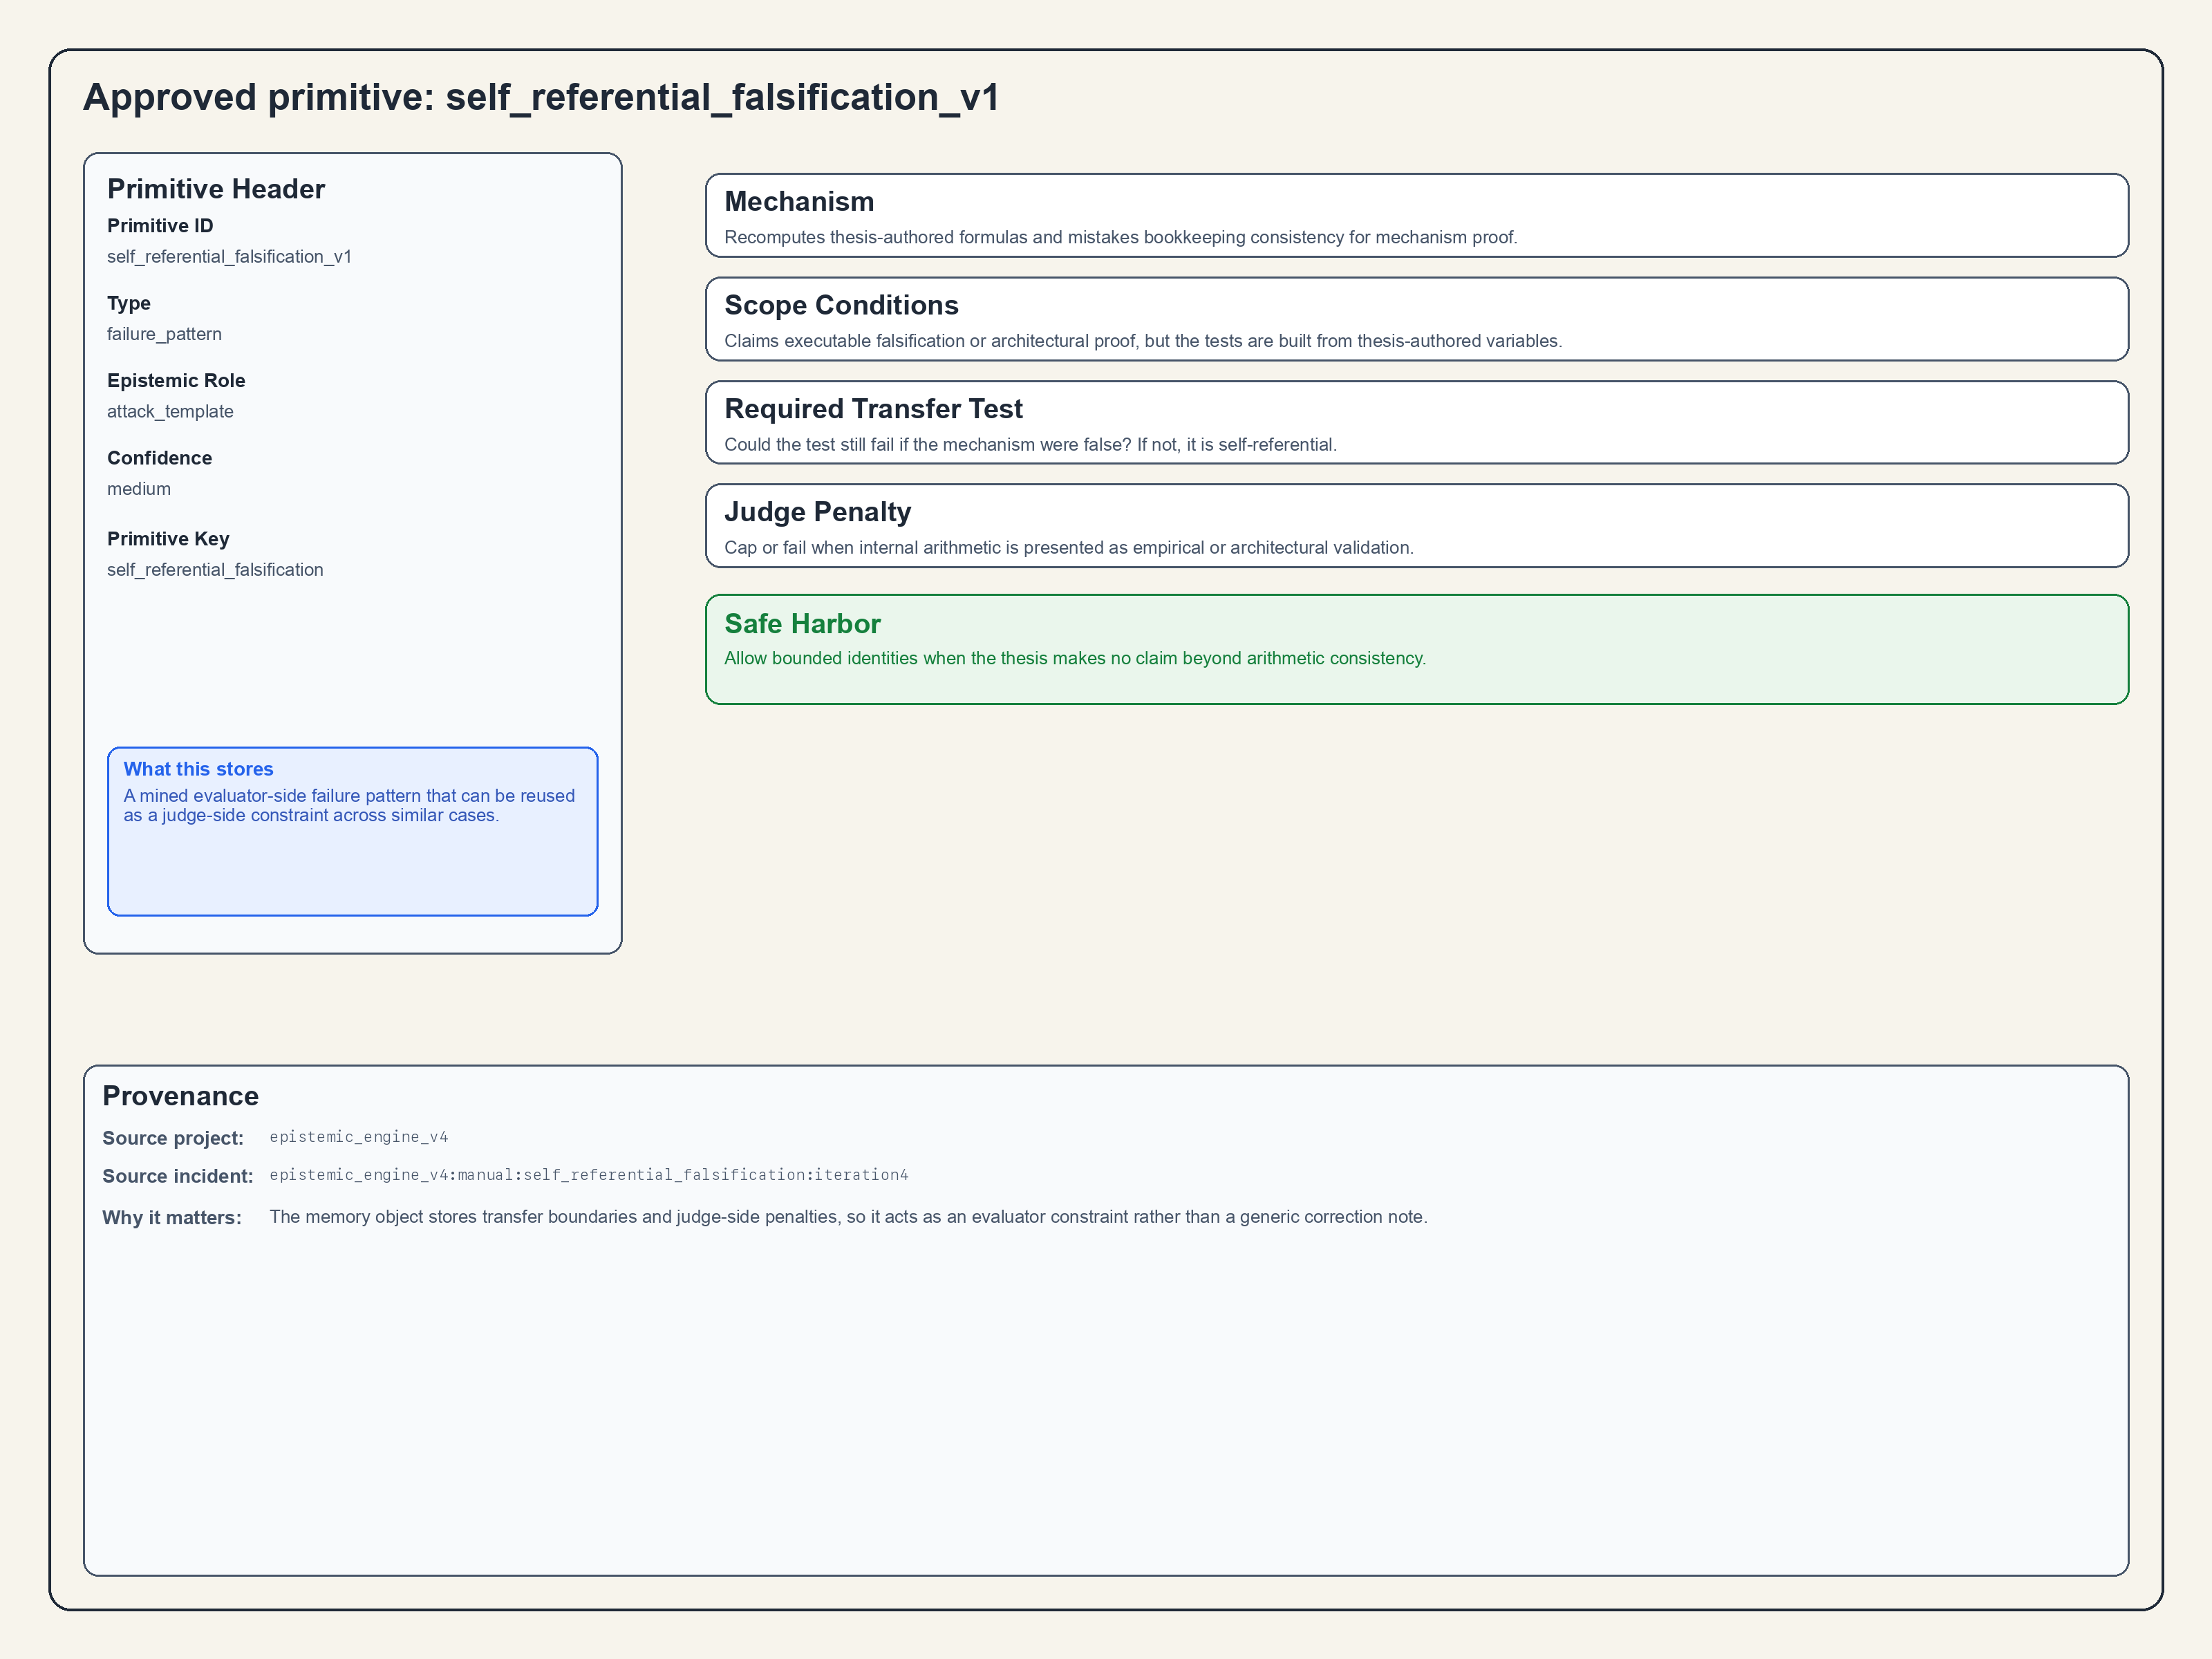
\includegraphics[width=\linewidth]{paper2_figure1.png}
  \caption{Example of an approved primitive (\texttt{self\_referential\_falsification\_v1}). Each primitive stores a failure family, transfer conditions, non-transfer boundaries, and judge-side penalty logic. This makes adversarial precedent memory a structured evaluator-hardening mechanism rather than a generic correction log.}
  \label{fig:primitive-schema}
\end{figure}

\subsubsection{2.3 Safe harbor}\label{23-safe-harbor}

Without calibration, adversarial memory overfires and kills bounded,
valid local components. Safe harbor rules preserve narrow deterministic
mappings that make only local claims and do not overclaim upstream
truthfulness.

\subsubsection{2.4 Evidence-Storage / Evaluator Separation}\label{24-aluram-separation}

Stateful evidence accumulation is allowed outside the evaluator, but the
validator remains stateless and zero-trust with respect to that state.
This is the architectural separation between evidence storage and
judgment.

\section{3. Benchmark Methodology}\label{3-benchmark-methodology}

The benchmark design is part of the paper\textquotesingle s
contribution. Because the system under test is semantic, the benchmark
must also be semantic-aware.

\subsubsection{3.1 Main suite}\label{31-main-suite}

The frozen main suite contains 10 specimens:

\begin{itemize}
\tightlist
\item
  8 bad specimens mined from historical runs across multiple exploit
  families
\item
  2 good controls representing bounded, valid local contracts
\end{itemize}

Benchmark conditions:

\begin{itemize}
\tightlist
\item
  \texttt{A\_baseline\_soft\_judge}
\item
  \texttt{B\_deterministic\_gates}
\item
  \texttt{C\_gates\_plus\_primitives}
\item
  \texttt{C2\_gates\_plus\_primitives\_crux\_first} (used only in later
  ablation runs)
\end{itemize}

\subsubsection{3.2 Claim-test-mismatch
mini-suite}\label{32-claim-test-mismatch-mini-suite}

A second suite isolates a narrower exploit family: tests that look
rigorous but prove scaffolding, tautologies, or peripheral math instead
of the load-bearing claim.

Historical specimens:

\begin{itemize}
\tightlist
\item
  \texttt{selective\_rigor\_recursive\_bayesian}
\item
  \texttt{selective\_rigor\_simulation\_god}
\item
  \texttt{tautological\_verification\_central\_station}
\end{itemize}

\subsubsection{3.3 Detection metrics}\label{33-detection-metrics}

We separate:

\begin{itemize}
\tightlist
\item
  \textbf{exploit-family detection}: did the evaluator identify the
  expected exploit family?
\item
  \textbf{fatal structural detection}: did it kill the thesis for a
  genuinely fatal structural reason, even if the family label differed?
\end{itemize}

This distinction was necessary because exact exploit taxonomy is brittle
while structural kill quality is the more stable empirical object.

\subsubsection{3.4 Semantic
adjudication}\label{34-semantic-adjudication}

Initial keyword matching created false negatives whenever the evaluator
paraphrased a correct diagnosis. We therefore added an adjudication
layer for semantic detection assessment. The adjudicator is measurement
infrastructure, not part of the evaluator itself.

One architectural caution emerged during auxiliary-case triage:
structural gates based on explicit test properties tend to be more
stable than semantic gates that require the LLM to make a binary
judgment call on an ambiguous pattern such as self-reference. We
therefore treat single-run outcomes driven by those semantic binary
gates as softer evidence unless they remain stable across reruns.

\subsubsection{3.5 Why the mini-suite
exists}\label{35-why-the-mini-suite-exists}

The claim-test-mismatch mini-suite is not a second copy of the main
benchmark. It isolates a specific exploit family where apparent rigor
hides a failure to test the crux. This suite is what later exposed a
blind spot in the primitive-conditioned evaluator itself.

\section{4. Results I: Gates And Utility On The Main
Suite}\label{4-results-i-gates-and-utility-on-the-main-suite}

The cleanest representative run from the frozen 10-specimen main suite
is \texttt{20260405\_090223}, which preserves the
\texttt{A\ -\textgreater{}\ B\ -\textgreater{}\ C} ladder after adding
\texttt{t6\_ai\_inference\_internal\_price\_floor}.

\subsubsection{\texorpdfstring{Table 1. Representative Main-Suite Run
(\texttt{20260405\_090223})}{Table 1. Representative Main-Suite Run (20260405\_090223)}}\label{table-1-representative-main-suite-run-20260405_090223}

\begin{table}[htbp]
\centering
\resizebox{\textwidth}{!}{%
\begin{tabular}{lrrrrrr}
\toprule
Condition & N & False Accept & False Reject & Family Detection & Structural Detection & Mean Good Score \\
\midrule
\texttt{A\_baseline\_soft\_judge} & 10 & 0.250 & 0.500 & 0.375 & 1.000 & 70.0 \\
\texttt{B\_deterministic\_gates} & 10 & 0.125 & 0.500 & 0.625 & 1.000 & 50.0 \\
\texttt{C\_gates\_plus\_primitives} & 10 & 0.000 & 0.000 & 0.625 & 1.000 & 100.0 \\
\bottomrule
\end{tabular}%
}
\end{table}

Interpretation:

\begin{itemize}
\tightlist
\item
  \texttt{B} fixes part of the score-channel problem but still falsely
  accepts one bad specimen.
\item
  \texttt{C} preserves the hardening while removing false rejects in
  this representative run.
\item
  the gain from \texttt{C} is best understood as
  \textbf{utility/calibration}, not just raw exploit detection.
\end{itemize}

\subsubsection{Mixed-family replication
summary}\label{mixed-family-replication-summary}

Across the frozen full 10-specimen main-suite reruns currently on disk
(\texttt{20260405\_090223}, \texttt{20260405\_091143},
\texttt{20260405\_092112}):

\begin{itemize}
\tightlist
\item
  \texttt{C} had lower false-accept rate than \texttt{B} in 1 run and
  tied in 2
\item
  \texttt{C} had lower false-reject rate than \texttt{B} in 2 runs and
  tied in 1
\item
  \texttt{C} had a higher mean good-specimen score in all 3 runs
\item
  average false-accept rate: \texttt{B\ =\ 0.125}, \texttt{C\ =\ 0.083}
\item
  average false-reject rate: \texttt{B\ =\ 0.333}, \texttt{C\ =\ 0.000}
\item
  average mean good score: \texttt{B\ =\ 64.67}, \texttt{C\ =\ 100.0}
\item
  average mean bad score: \texttt{B\ =\ 15.63}, \texttt{C\ =\ 10.42}
\item
  average structural detection rate: \texttt{B\ =\ 0.958},
  \texttt{C\ =\ 0.958}
\end{itemize}

The dominant remaining bad-case instability is
\texttt{t2\_ai\_inference}: \texttt{B} falsely accepted it in all three
frozen reruns, while \texttt{C} caught it once and missed it twice. That
instability narrows the strength of any single-run narrative, but it
does not change the overall utility pattern on the frozen benchmark.

By contrast, the newly promoted
\texttt{t6\_ai\_inference\_internal\_price\_floor} behaved cleanly
across all three frozen runs: \texttt{A} falsely accepted it every time,
while both \texttt{B} and \texttt{C} rejected it every time. That
specimen is therefore the clearest stable demonstration of the
\texttt{A\ -\textgreater{}\ B} hardening step on the frozen benchmark.

This supports a conservative result statement: \textbf{adversarial
precedent memory improved the default utility of the evaluator across
repeated post-calibration runs, but did not uniformly dominate on every
run or metric.}

\section{\texorpdfstring{5. Results II: Ordering Ablation (\texttt{C}
vs
\texttt{C2})}{5. Results II: Ordering Ablation (C vs C2)}}\label{5-results-ii-ordering-ablation-c-vs-c2}

The ordering question arose only after the evaluator benchmark exposed a
self-blind spot.

\subsubsection{\texorpdfstring{Table 2A. Discovery Run}{Table 2A. Discovery Run}}\label{table-2a-discovery-run}

\begin{table}[htbp]
\centering
\resizebox{\textwidth}{!}{%
\begin{tabular}{lrrrr}
\toprule
Condition & N & False Accept & Family Detection & Structural Detection \\
\midrule
\texttt{A\_baseline\_soft\_judge} & 3 & 1.000 & 0.333 & 0.667 \\
\texttt{B\_deterministic\_gates} & 3 & 0.333 & 0.667 & 0.667 \\
\texttt{C\_gates\_plus\_primitives} & 3 & 0.333 & 0.667 & 1.000 \\
\bottomrule
\end{tabular}%
}
\end{table}

This run is the blind-spot discovery. \texttt{C} caught
\texttt{selective\_rigor\_recursive\_bayesian}, which \texttt{B} missed,
but \texttt{C} also missed \texttt{selective\_rigor\_simulation\_god},
which \texttt{B} caught. That cross-over is what triggered the
architectural diagnosis. The run ID is
\texttt{20260404\_213459}.

\subsubsection{\texorpdfstring{Table 2B. Crux-First Ablation}{Table 2B. Crux-First Ablation}}\label{table-2b-crux-first-ablation}

\begin{table}[htbp]
\centering
\resizebox{\textwidth}{!}{%
\begin{tabular}{lrrrr}
\toprule
Condition & N & False Accept & Family Detection & Structural Detection \\
\midrule
\texttt{A\_baseline\_soft\_judge} & 3 & 0.667 & 0.333 & 1.000 \\
\texttt{B\_deterministic\_gates} & 3 & 0.333 & 0.667 & 0.667 \\
\texttt{C\_gates\_plus\_primitives} & 3 & 0.667 & 0.333 & 0.667 \\
\texttt{C2\_gates\_plus\_primitives\_crux\_first} & 3 & 0.000 & 1.000 & 1.000 \\
\bottomrule
\end{tabular}%
}
\end{table}

This run tests the targeted repair. \texttt{C2} cleans up the
claim-test-mismatch suite, but the varying \texttt{C} column across the
two mini-suite runs makes the stochasticity visible rather than hiding
it. The run ID is \texttt{20260404\_221606}.

\subsubsection{\texorpdfstring{Table 2C. Main Suite With \texttt{C2}
(\texttt{20260404\_223826}, pre-freeze \texttt{N=9}
ablation)}{Table 2C. Main Suite With C2 (20260404\_223826, pre-freeze N=9 ablation)}}\label{table-2c-main-suite-with-c2-20260404_223826-pre-freeze-n9-ablation}

\begin{table}[htbp]
\centering
\resizebox{\textwidth}{!}{%
\begin{tabular}{lrrrrrr}
\toprule
Condition & N & False Accept & False Reject & Family Detection & Structural Detection & Mean Good Score \\
\midrule
\texttt{B\_deterministic\_gates} & 9 & 0.143 & 0.500 & 0.571 & 1.000 & 44.0 \\
\texttt{C\_gates\_plus\_primitives} & 9 & 0.000 & 0.500 & 1.000 & 1.000 & 37.5 \\
\texttt{C2\_gates\_plus\_primitives\_crux\_first} & 9 & 0.143 & 0.500 & 0.571 & 1.000 & 50.0 \\
\bottomrule
\end{tabular}%
}
\end{table}

This is the generalization test. \texttt{C2} fixes the mini-suite but
does not beat \texttt{C} as the broader default condition. In this run
it reintroduced the \texttt{t2\_ai\_inference} false accept that
\texttt{C} had eliminated.

The resulting empirical law is narrower than "crux-first is better":
\textbf{primitive-ordering gains are exploit-family-specific rather than
uniformly dominant.}

\section{6. Results III: The Evaluator Surfaced Its Own Blind
Spot}\label{6-results-iii-the-evaluator-surfaced-its-own-blind-spot}

The most distinctive result is not a single metric table but a process
trace.

\subsubsection{\texorpdfstring{Step 1: Blind-spot discovery
(\texttt{20260404\_213459})}{Step 1: Blind-spot discovery (20260404\_213459)}}\label{step-1-blind-spot-discovery-20260404_213459}

On the claim-test-mismatch suite:

\begin{itemize}
\tightlist
\item
  \texttt{selective\_rigor\_recursive\_bayesian}

  \begin{itemize}
  \tightlist
  \item
    \texttt{B}: passed at \texttt{100}
  \item
    \texttt{C}: failed at \texttt{0}
  \end{itemize}
\item
  \texttt{selective\_rigor\_simulation\_god}

  \begin{itemize}
  \tightlist
  \item
    \texttt{B}: failed at \texttt{25}
  \item
    \texttt{C}: passed at \texttt{100}
  \end{itemize}
\end{itemize}

The key point is that the score contract was not broken. The detection
flags changed. Primitive conditioning helped on one specimen and hurt on
another.

\subsubsection{Step 2: Architectural
diagnosis}\label{step-2-architectural-diagnosis}

The diagnosis was that front-loaded primitives could bias the
evaluator\textquotesingle s first reading of the crux. That produced a
new constraint:

\begin{itemize}
\tightlist
\item
  identify the load-bearing claim first
\item
  determine whether the test suite targets that claim
\item
  only then inject precedent memory
\end{itemize}

\subsubsection{\texorpdfstring{Step 3: Follow-up ablation
(\texttt{20260404\_221606})}{Step 3: Follow-up ablation (20260404\_221606)}}\label{step-3-follow-up-ablation-20260404_221606}

The new \texttt{C2\_gates\_plus\_primitives\_crux\_first} condition
repaired the missed \texttt{simulation\_god} case and cleaned up the
mini-suite.

\subsubsection{\texorpdfstring{Step 4: Generalization test
(\texttt{20260404\_223826})}{Step 4: Generalization test (20260404\_223826)}}\label{step-4-generalization-test-20260404_223826}

\texttt{C2} did not become the new default winner on the full suite. It
solved one exploit-family problem and reopened another.

Figure~\ref{fig:recursive-loop} summarizes this sequence.

This is the paper\textquotesingle s strongest methodology result:

\begin{itemize}
\tightlist
\item
  the evaluation infrastructure surfaced its own blind spot
\item
  humans converted that failure into a new architectural constraint
\item
  the new constraint was then tested directly
\end{itemize}

This is not autonomous self-improvement. It is a reproducible
human-in-the-loop method for recursive evaluator hardening.

\begin{figure}[htbp]
  \centering
  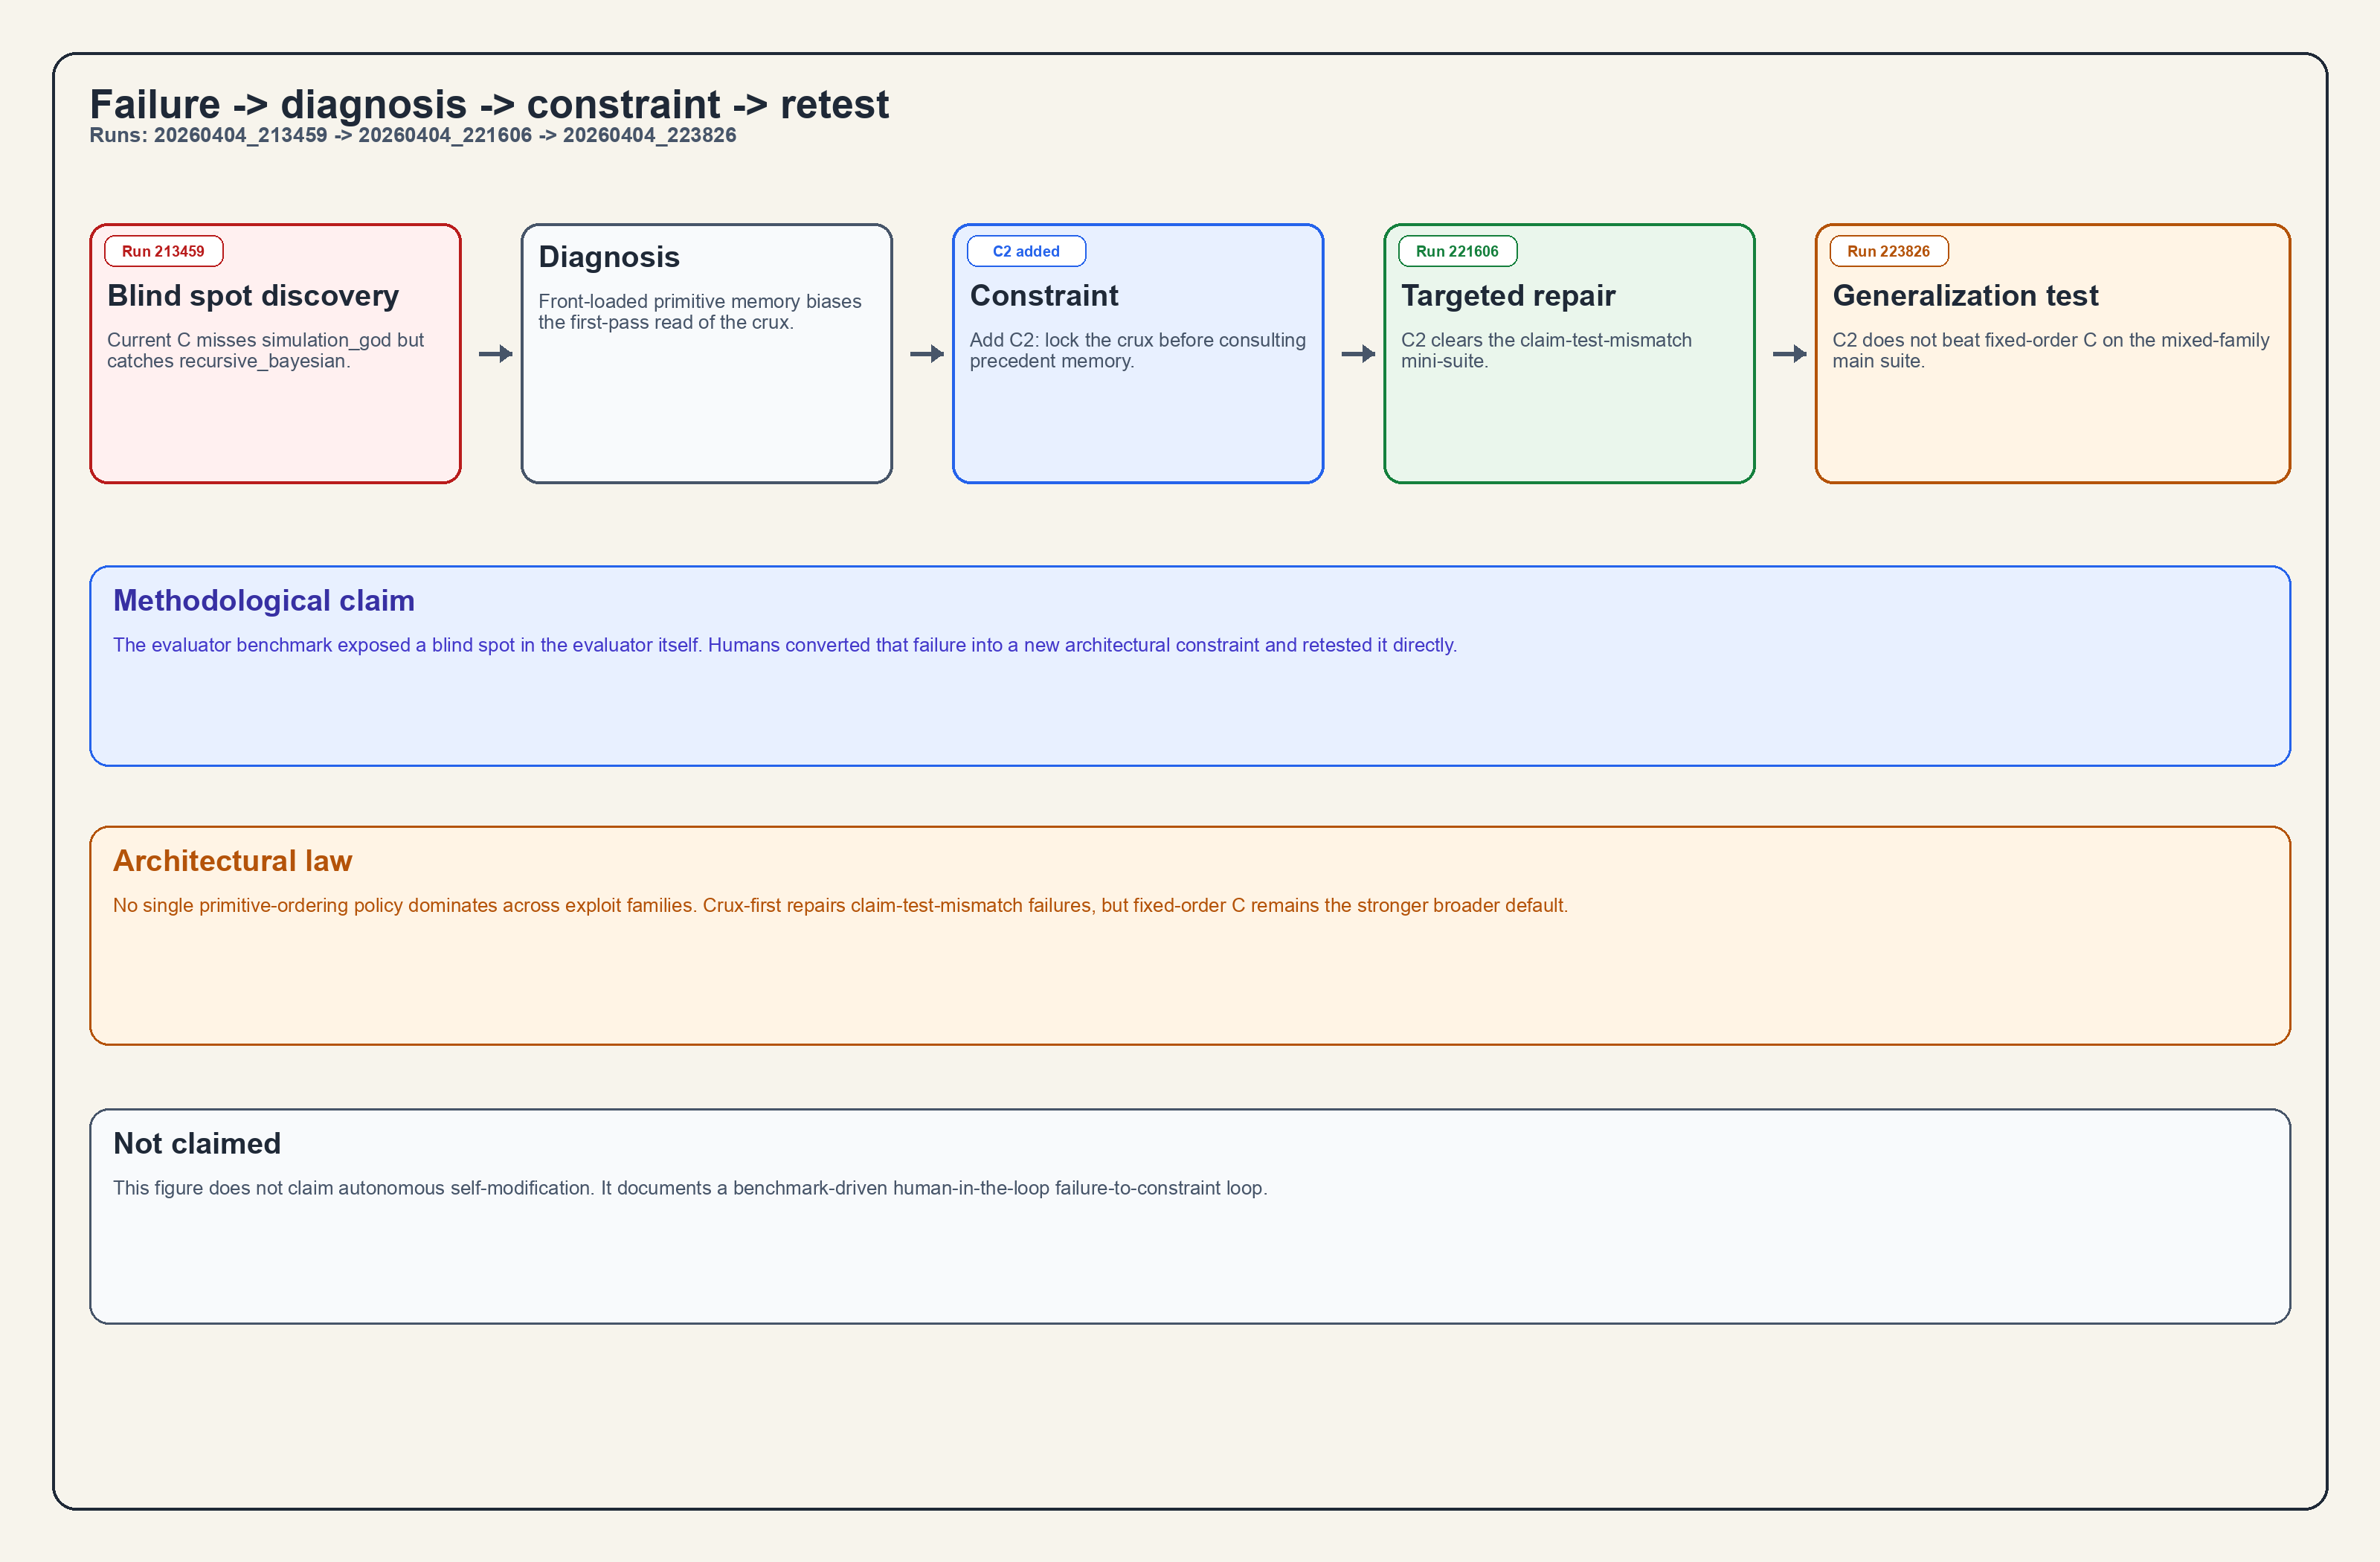
\includegraphics[width=\linewidth]{paper2_figure2.png}
  \caption{Benchmark-driven recursive hardening of the evaluator. A claim-test-mismatch benchmark exposed a primitive-ordering blind spot (\texttt{20260404\_213459}), which was diagnosed as front-loaded precedent bias. That diagnosis became a new crux-first constraint (\texttt{C2}), which repaired the narrow exploit family (\texttt{20260404\_221606}) but did not dominate on the broader main suite (\texttt{20260404\_223826}).}
  \label{fig:recursive-loop}
\end{figure}

\section{7. Discussion}\label{7-discussion}

\subsubsection{7.1 What the paper actually
shows}\label{71-what-the-paper-actually-shows}

The paper does \textbf{not} show that one hardened pipeline universally
dominates. It shows:

\begin{itemize}
\tightlist
\item
  deterministic gates reduce reward-channel corruption
\item
  adversarial precedent memory improves default utility on a
  mixed-family benchmark
\item
  ordering benefits are exploit-family-specific
\item
  evaluator failures can be converted into new evaluator constraints
  through a structured loop
\end{itemize}

\subsubsection{7.2 Constraint vs
correction}\label{72-constraint-vs-correction}

This system does not store a verbal note saying "do better next time."
It stores adversarial precedents with scope, transfer, and penalty
logic. That makes the memory object different from a generic correction
log. A correction tries to pull the model toward a positive target; an
adversarial constraint acts as a family-specific floor that prevents a
known vector of ruin from being paid twice.

\subsubsection{7.3 Why Goodhart belongs
here}\label{73-why-goodhart-belongs-here}

The score-channel problem is a reward-target problem. More subtly, the
ordering-ablation result shows that hardening one layer can move failure
modes rather than erase them. Goodhart is therefore a useful supporting
theoretical lens \citep{manheim2019goodhart}, though not the paper\textquotesingle s central
framing.

\subsubsection{7.4 Design implication: from fixed ordering to
family-aware
routing}\label{74-design-implication-from-fixed-ordering-to-family-aware-routing}

These results establish the prerequisite for family-aware primitive
routing. Fixed-ordering pipelines do not uniformly dominate across
exploit families: the same ordering change that repairs
claim-test-mismatch failures can reopen a different mixed-family blind
spot. The next architecture should therefore move away from a single
global primitive order and toward routing constraints based on the
detected exploit family.

\subsubsection{7.5 Limitations}\label{75-limitations}

\begin{itemize}
\tightlist
\item
  small benchmark (\texttt{N=10} main, \texttt{N=3} mini)
\item
  stochastic LLM judge variance, including visible run-to-run variation
  in mini-suite \texttt{C} performance
\item
  human-in-the-loop redesign rather than autonomous evaluator
  self-modification
\item
  benchmark coverage is broad enough to be informative, but not broad
  enough for universal claims
\end{itemize}

\subsubsection{7.6 Threats to validity}\label{76-threats-to-validity}

To keep the empirical claims bounded by the evidence, five threats
matter most.

\textbf{Small specimen count.} The benchmark is intentionally narrow.
False-accept and false-reject rates on \texttt{N=10} and \texttt{N=3} do
not carry large-sample statistical authority and should not be read as
universal laws of LLM evaluation. They function here as auditable
systems traces on a curated mixed-family suite.

\textbf{Judge stochasticity.} The evaluator is non-deterministic, so
single-run wins are not sufficient evidence of stable superiority. This
is why the paper reports a post-calibration replication summary across
repeated main-suite runs and treats the \texttt{C\ \textgreater{}\ B}
result as a directional utility claim rather than a universal dominance
claim.

\textbf{Binary gate variance.} In one auxiliary specimen, the binary
gate assessment \texttt{proof\_is\_self\_referential} flipped between
runs under identical conditions, producing a
\texttt{25\ -\textgreater{}\ 100} score swing. This is more serious than
ordinary score jitter because it changes the gate path itself. For
specimens whose gaming signal lies near the LLM gate\textquotesingle s
semantic detection threshold, individual run outcomes should therefore
not be treated as stable benchmark evidence. The main benchmark
specimens were selected partly on repeated-run stability; auxiliary
specimens did not undergo the same stability filter.

The clearest frozen-main-suite instance of this is
\texttt{t2\_ai\_inference}. \texttt{B} missed \texttt{t2} in all three
frozen reruns, which is a systematic gate failure rather than
stochasticity. \texttt{C} caught \texttt{t2} once and missed it twice,
which is a separate phenomenon: semantic-gate variance near the
detection threshold. We therefore distinguish stable gate blind spots
from run-to-run LLM detection variance when interpreting bad-case
failures.

\textbf{Human-in-the-loop diagnosis.} The transition from benchmark
anomaly to architectural constraint was performed by a human systems
designer. The paper therefore demonstrates a reproducible hardening
methodology, not an autonomous recursive self-improvement algorithm.

\textbf{Exploit-family annotation dependence.} Taxonomic labels such as
\texttt{selective\ rigor}, \texttt{tautological\ verification}, or
\texttt{claim-test\ mismatch} involve judgment. To reduce dependence on
taxonomy alone, the core empirical claims rely primarily on structural
kill outcomes and on transparent run-level examples rather than on
exploit-family naming accuracy by itself.

\textbf{Co-evolution of benchmark and system.} The benchmark and
evaluator were calibrated together, especially around good-control safe
harbor. Early autoimmune runs are part of the design history but are
separated from the post-calibration replication summary so that distinct
architectural regimes are not mixed inside the same empirical claim.

\subsubsection{7.7 Held-out stress checks and auxiliary
evidence}\label{77-held-out-stress-checks-and-auxiliary-evidence}

The out-of-domain logistics specimen was useful as a held-out stress
check but not as a primitive-specific wedge. In both iterations of that
specimen, all three conditions rejected the thesis. This shows that the
evaluator did not collapse outside the historical benchmark domains, but
it does \textbf{not} isolate precedent-memory transfer advantage because
the deterministic gates found conventional structural kill paths before
any \texttt{domain\_leakage}-specific distinction became decisive.

The auxiliary historical suite also remained auxiliary by design. One
case, \texttt{central\_station\_hypothetical\_target\_laundering},
showed directional \texttt{B\ -\textgreater{}\ C} lift in a mixed
auxiliary run (\texttt{A=59}, \texttt{B=25}, \texttt{C=0}), but it
failed the stability bar for promotion when rerun in isolation
(\texttt{A=59}, \texttt{B=100}, \texttt{C=100}). Another case,
\texttt{central\_station\_mirrored\_monte\_carlo}, also flipped across
runs. We therefore use these auxiliary results only as robustness and
variance observations, not as additional core benchmark specimens.

\subsubsection{7.8 Future work: adversarial traces as process-supervision data}\label{78-future-work-adversarial-traces-as-process-supervision-data}

The primary contribution of this paper is test-time hardening for
strategic and financial reasoning, not a training-time algorithmic
advance. But the ZTARE pipeline also emits structured adversarial
traces: persuasive but structurally flawed trajectories that fail under
execution, and surviving trajectories that withstand adversarial
pressure.

Those paired traces have the right shape for future process-supervision
work in domains where objective reward signals are otherwise weak. In
principle, they could support supervised contrastive datasets,
evaluator-training corpora, or future Process Reward Model work
targeted at complex strategic reasoning.

We do not claim that the current corpus is sufficient for competitive
reinforcement learning or frontier PRM training. At present, the scale
is only enough to demonstrate the architectural possibility of
execution-backed trace generation. The present paper's contribution
remains the hardening of test-time evaluation; large-scale distillation
of these traces into training-time systems is future work.

\section{8. Related Work}\label{8-related-work}

The relevant contrast points are:

\begin{enumerate}
\def\labelenumi{\arabic{enumi}.}
\tightlist
\item
  \textbf{Constraint vs correction.} Reflexion- and
  self-refinement-style systems store corrections or feedback traces
  \citep{shinn2023reflexion,madaan2023selfrefine}. This work stores
  adversarial constraints.
\item
  \textbf{Mined vs authored.} Constitutional-style rules are
  hand-authored \citep{bai2022constitutional}. Here the constraints are
  mined from observed evaluator and thesis failures.
\item
  \textbf{Evaluator vs generator attachment.} The memory is attached to
  the evaluator and used to harden judgment against recurrent exploit
  families, not simply to improve generation quality.
\end{enumerate}

This paper also connects to:

\begin{itemize}
\tightlist
\item
  reward hacking / Goodhart literature \citep{manheim2019goodhart}
\item
  LLM-as-judge reliability literature \citep{zheng2023judging,verga2024replacing}
\item
  adversarial evaluation and debate systems \citep{perez2022red,irving2018debate}
\end{itemize}

The closest adjacent literature studies when LLM judges are reliable,
how evaluator bias appears, and which judge configurations correlate
best with human preference or task success \citep{zheng2023judging,verga2024replacing}. This paper asks a different
question: how can evaluator reliability be improved through structural
hardening? The contribution here is therefore not another diagnosis of
judge failure, but an empirical hardening pipeline built from
deterministic gates, adversarial precedent memory, and ordering
ablations that expose when those hardening layers help or interfere.

\bibliographystyle{plainnat}
\bibliography{refs}

\appendix
\section{Appendix A1. Main-Suite Replication
Table}\label{appendix-a1-main-suite-replication-table}

Only frozen full 10-specimen main-suite runs are included.

\begin{landscape}
\begin{table}[htbp]
\centering
\small
\resizebox{\linewidth}{!}{%
\begin{tabular}{lrrrrrrrr}
\toprule
Run ID & B FA & C FA & B FR & C FR & B Mean Good & C Mean Good & B Str. Det. & C Str. Det. \\
\midrule
\texttt{20260405\_090223} & 0.125 & 0.000 & 0.500 & 0.000 & 50.0 & 100.0 & 1.000 & 1.000 \\
\texttt{20260405\_091143} & 0.125 & 0.125 & 0.500 & 0.000 & 50.0 & 100.0 & 0.875 & 0.875 \\
\texttt{20260405\_092112} & 0.125 & 0.125 & 0.000 & 0.000 & 94.0 & 100.0 & 1.000 & 1.000 \\
\textbf{Average} & \textbf{0.125} & \textbf{0.083} & \textbf{0.333} & \textbf{0.000} & \textbf{64.67} & \textbf{100.0} & \textbf{0.958} & \textbf{0.958} \\
\bottomrule
\end{tabular}%
}
\end{table}
\noindent\textit{Legend.} FA = false accept, FR = false reject, Str. Det. = structural detection.
\end{landscape}

\textbf{Footnote.} Earlier \texttt{N=9} runs are retained as design
history and pre-freeze ablation context, but they are excluded from this
appendix because the frozen main benchmark now includes
\texttt{t6\_ai\_inference\_internal\_price\_floor} and is therefore a
distinct evaluation regime.

\end{document}
